\newpage
\subsection{Naked Subset}
Die Technik \textit{Naked Subset} ist ein Überbegriff für die Techniken \textit{Naked Pair}, \textit{Naked Triple} und \textit{Naked Quadruple}. Alle Techniken Arbeiten nach dem selben Prinzip, der Unterschied liegt in der Anzahl der verwendeten Kandidatenlisten. Bei \textit{NakedSubsets} sucht man nach Paaren, Tripeln oder Quadrupeln von Zellen in Figuren, nach Kandidatenlisten einer bestimmten Eigenschaft. Die Vereinigung der Listen muss eine bestimmte Anzahl Elemente enthalten. Bei Paaren sind das zwei, bei Tripeln drei und bei Quadrupeln vier Einträge in den Kandidatenlisten.\\
Findet man zum Beispiel ein Paar, das nur noch die selben beiden Zahlen enthalten kann dann ist klar, dass keine der Zahlen anderswo in der Figur stehen kann, da sonst für eine der Zellen keine Zahl mehr übrig bleibt. Daher können die beiden Zahlen dann aus den Kandidatenlisten aller anderen Zahlen aus der Figur entfernt werden.
Die Begründung für Tripel und Quadrupel ist analog.\\
Es ist nicht nötig nach mehr als Quadrupeln zu suchen, da für jedes Naked Quintupel ein Hidden Quadrupel existiert.

\begin{figure}[h]
\begin{center}
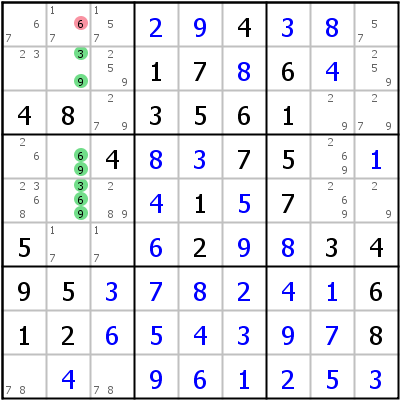
\includegraphics{./img/naked_subset.png}
\caption{Naked Subset - Naked Triple}
\end{center}
\end{figure}

In \textbf{Abbildung 2.8} findet man das \textit{Naked Subset} in Zeile 2. Genauer gesagt handelt es sich um ein \textit{Naked Triple}. Hier hat die Vereinigung der Kandidatenlisten der Zellen z2s5, z2s6 und z2s8 genau drei Einträge: 1, 3 und 7. Es gibt offensichtlich keine andere Möglichkeit, als die drei Ziffer auf diese zellen zu verteilen. Demnach können sie in der Zeile sonst nicht vorkommen und können aus den Kandidatenlisten der anderen Zellen entfernt werden.
